\documentclass[english]{tudscrreprt}
\usepackage[T1]{fontenc}
%\usepackage[ngerman=ngerman-x-latest]{hyphsubst}
\usepackage{babel}
\usepackage{isodate}
\usepackage{tudscrsupervisor}
\usepackage{enumitem}\setlist{noitemsep}
\usepackage{siunitx}
\usepackage{tabto}

\begin{document}
\faculty{Faculty of Electrical and Computer Engineering}
\institute{Institute of Electrical Power Engineering}\chair{Chair of Electromagnetic Theory and Compatibility}
\title{%
Large Reverberation Chamber
}\date{\today}
\contactperson{%
Prof. Hans Georg Krauthäuser\emailaddress{tetemv@tu-dresden.de}
\office{Görges-Bau, Room 223}\telephone{+49 351 463-33357}
%\and%
%Mac Moneysac\emailaddress{mac.moneysac@tu-dresden.de}
%\office{Dingens-Bau, Zimmer~15}\telephone{+49 351 463-54321}
}
\noticeform[headline=Laboratory Description,pagestyle=empty]{%
  \renewcommand{\focusname}{Parameter}
  \renewcommand{\contactpersonname}{Contact Person}
 Reverberation chambers are alternative test environments to free fields and anechoic chambers.

In addition to a range of special applications, classic EMC interference emission and immunity tests as well as measurements on shielding attenuation and transfer functions can be carried out here in accordance with international standards. The particular advantage in the area of immunity is that very high field strengths can be achieved. Overall, measurements in reverberation chambers prove to be very robust in terms of high reproducibility in the same or other similar measurement environments.  
\begin{center}
  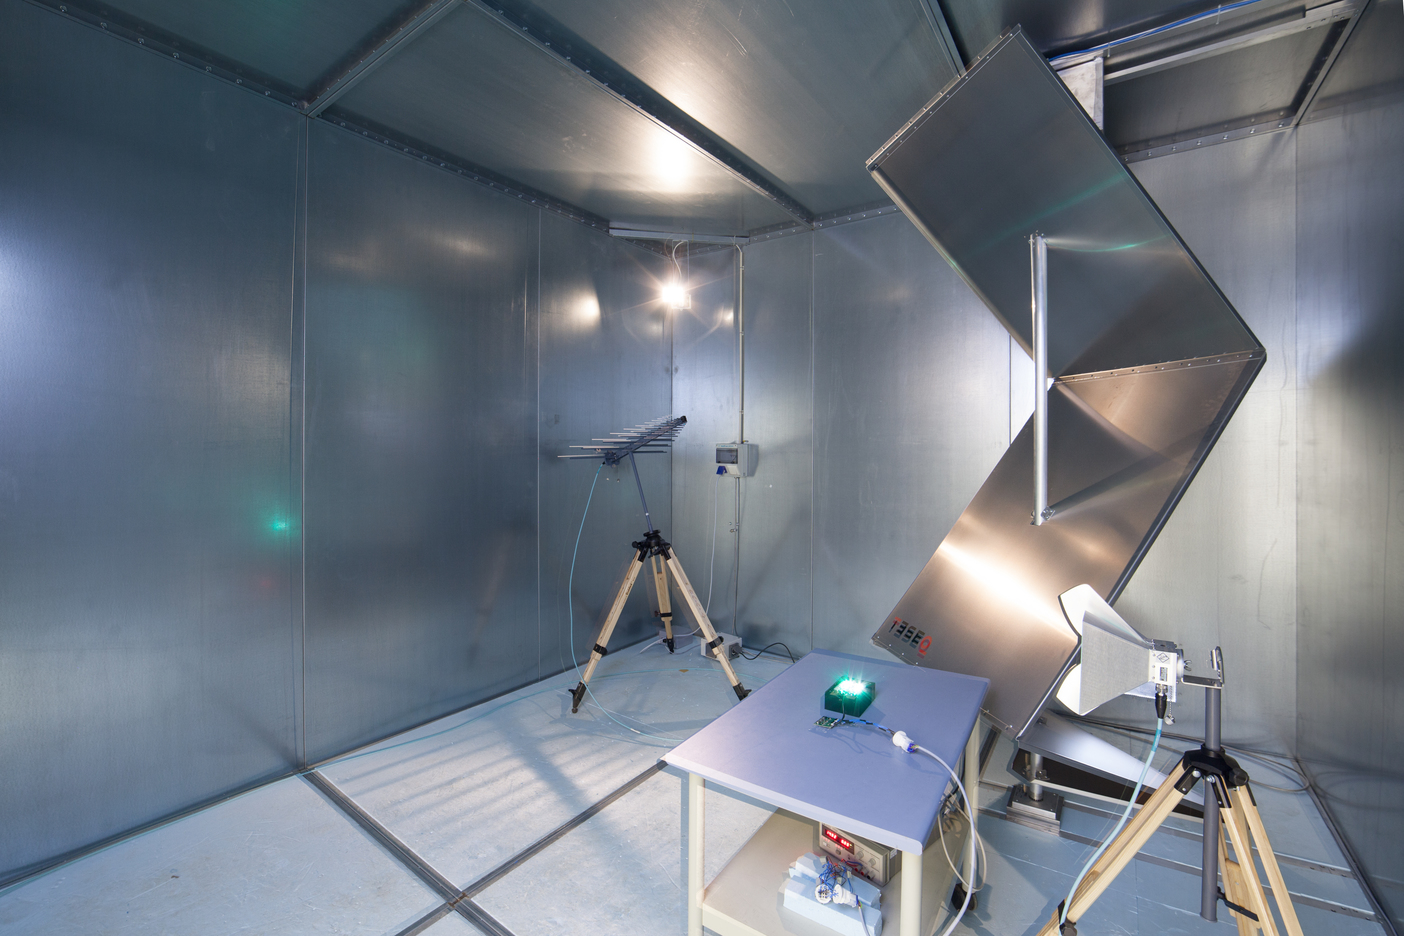
\includegraphics[width=.45\linewidth]{mvk_innenraum_klein}
  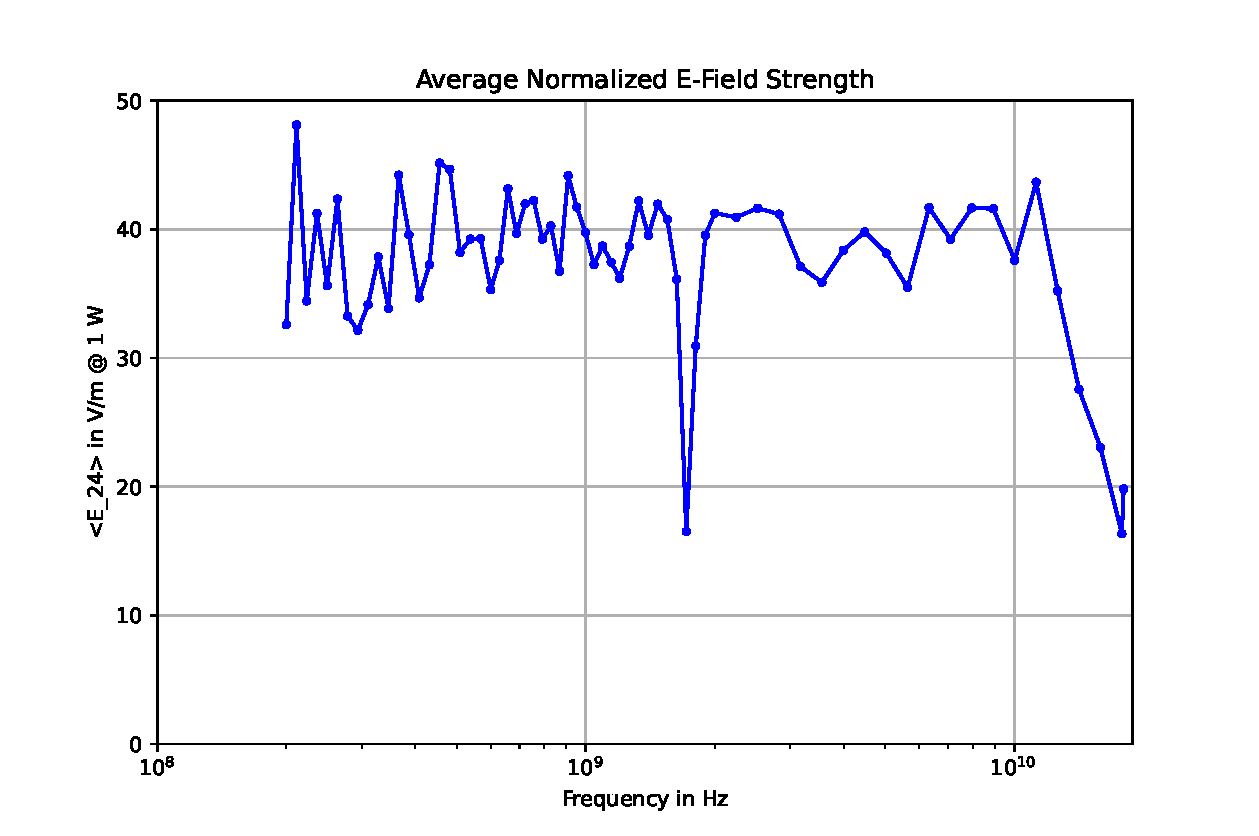
\includegraphics[width=.52\linewidth]{E24}
\renewcommand*{\figureformat}{Left}
\captionof{figure}{View of the Large Reverberation Chamber. Right: Field Strength @ \qty{1}{\watt}}
\end{center}
}{%
\item Frequency range:\tabto{.3\linewidth} \qtyrange{0.2}{18}{\giga\hertz}
\item Field Strength: \tabto{.3\linewidth} $>$ \qty{100}{\volt\per\metre}
\item Size ($l \times w \times h$): \tabto{.3\linewidth} $\qty{5.3}{\metre} \times \qty{3.7}{\metre} \times \qty{3.0}{\metre}$
\item Available Power: \tabto{.3\linewidth} \qtyrange{80}{2000}{\mega\hertz}: \qty{100}{\watt}\\
  \tabto{.3\linewidth} \qtyrange{2}{6}{\giga\hertz}: \qty{30}{\watt}\\
  \tabto{.3\linewidth} \qtyrange{6}{18}{\giga\hertz}: \qty{20}{\watt}
\item Main Standards:
  \begin{itemize}
  \item IEC~61000-4-21, EN~61000-4-21, DIN~EN~61000-4-21
    \item RTCA DO-160
    \item MIL-STD-461
    \end{itemize}
}
\end{document}